\documentclass[../../../main.tex]{subfiles}
\begin{document}
\subsection*{Appendix I: Ohm's Law}
\subsection*{Example 1.} Two long coaxial metal cylinders (radii $a$ and $b$) are separated by material of conductivity $\sigma$. If they are maintained at a potential difference $V$, what current flows from one to the other, in a length $L$?

First we need to determine the Field. Using Gauss' Theorem,
\begin{align*}
    \oint \mathbf{E}&=\frac{Q_\text{enc}}{\epsilon_0}\\
    E2\pi sL&=\frac{\lambda L}{\epsilon_0}\\
\end{align*}
thus
\begin{equation*}
    \mathbf{E}=\frac{\lambda}{2\pi s\epsilon_0}\mathbf{\hat{s}}
\end{equation*}
While current is
\begin{equation*}
    I=\int \mathbf{J}\cdot d\mathbf{a}=\int \sigma\mathbf{E}\cdot d\mathbf{a}=\frac{\sigma}{\epsilon_0}\lambda L
\end{equation*}
and the potential difference between the cylinders is
\begin{align*}
    V(a)-V(b)=V=-\int_{b}^{a}\mathbf{E}\cdot d\mathbf{l}=\frac{\lambda}{2\pi\epsilon_0}\ln \frac{b}{a}
\end{align*}
so
\begin{equation*}
    I=\frac{2\pi\sigma L}{\ln b/a}V
\end{equation*}
\begin{figure*}[h]
    \centering
    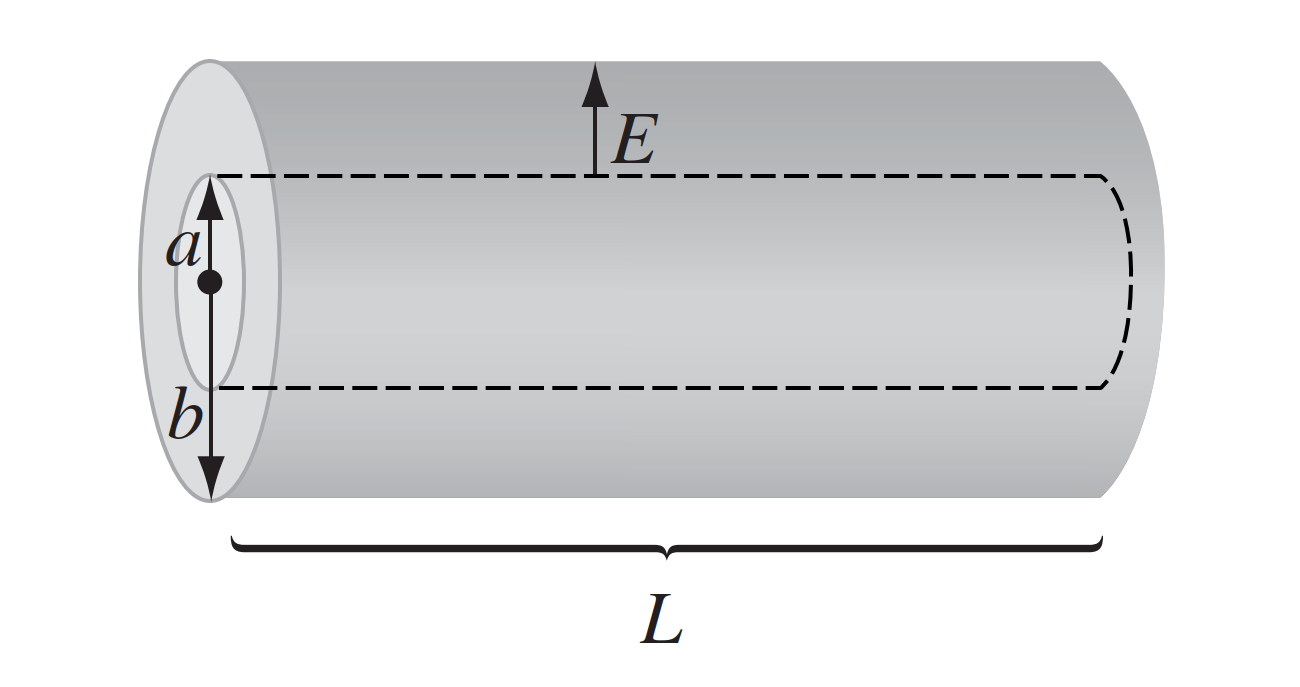
\includegraphics[width=0.5\textwidth]{../Rss/Electromagnetism/Electrodynamics/Ohm.png}
\end{figure*}

\subsection*{Appendix II: Circuits}
\subsubsection*{Impedance.} For resistor, impedance, or rather resistance, is defined by Ohm's Law (derivated) 
\begin{equation*}
    R=\frac{V}{I}
\end{equation*}
We define capacitive reactance as:
\begin{equation*}
    X_C=-i\frac{1}{2\pi fC}
\end{equation*}
The inductive reactance can be found using:
\begin{equation*}
    X_L=i2\pi f L
\end{equation*}

\subsubsection*{Resonance.} This phenomenon occurs when our circuit has maximum value of current, which resulted from having minimum impedance. Since minimum impedance occur when $X_L=X_C$,
\begin{equation*}
    f=\frac{1}{2\pi\sqrt{LC}}
\end{equation*}

\subsubsection*{RC Circuits.} Applying Kirchhoff’s loop rule to the circuit after the switch is thrown to position $a$, we get 
\begin{align*}
    iR+\frac{1}{C}q&=\upvarepsilon\\
    \dot{q}+\frac{1}{RC}q&=\frac{\upvarepsilon}{R}
\end{align*}
this is first order ODE, which can be easily solved using integral factor
\begin{equation*}
    I=\int \frac{1}{RC}dt=\frac{t}{RC}
\end{equation*} 
Then
\begin{align*}
    q&=e^{-t/RC}\int \frac{\upvarepsilon}{R}e^{t/RC}\;dt+Ae^{-t/RC}\\
    q&=C\upvarepsilon+Ae^{-t/RC}
\end{align*}
Applying boundary condition $q(0)=0$, we get $A=-C\upvarepsilon$, thus 
\begin{equation*}
    q=C\upvarepsilon(1-e^{-t/RC})
\end{equation*}
Since $i=dq/dt$
\begin{equation*}
    i=\frac{\upvarepsilon}{R}e^{-t/RC}
\end{equation*}
Time constant $\tau\equiv RC$ of the circuit represents the time interval during which the current decreases to $1/e$ of its initial value. Now, imagine that the capacitor is completely charged. If the switch is now thrown to position b, the capacitor begins to discharge through the resistor. The differential equation becomes
\begin{equation*}   
    \dot{q}+\frac{1}{RC}q=0
\end{equation*}
with general solution 
\begin{equation*}
    q=Ae^{-t/RC}
\end{equation*}
Applying boundary condition $q(0)=Q_i$, we get $A=Q_i$, thus 
\begin{equation*}
    q=Q_ie^{-t/RC}
\end{equation*}
As for the instantaneous current
\begin{equation*}
i=-\frac{Q_i}{RC}e^{-t/RC}=-I_ie^{-t/RC}
\end{equation*}
\begin{figure*}
    \centering
    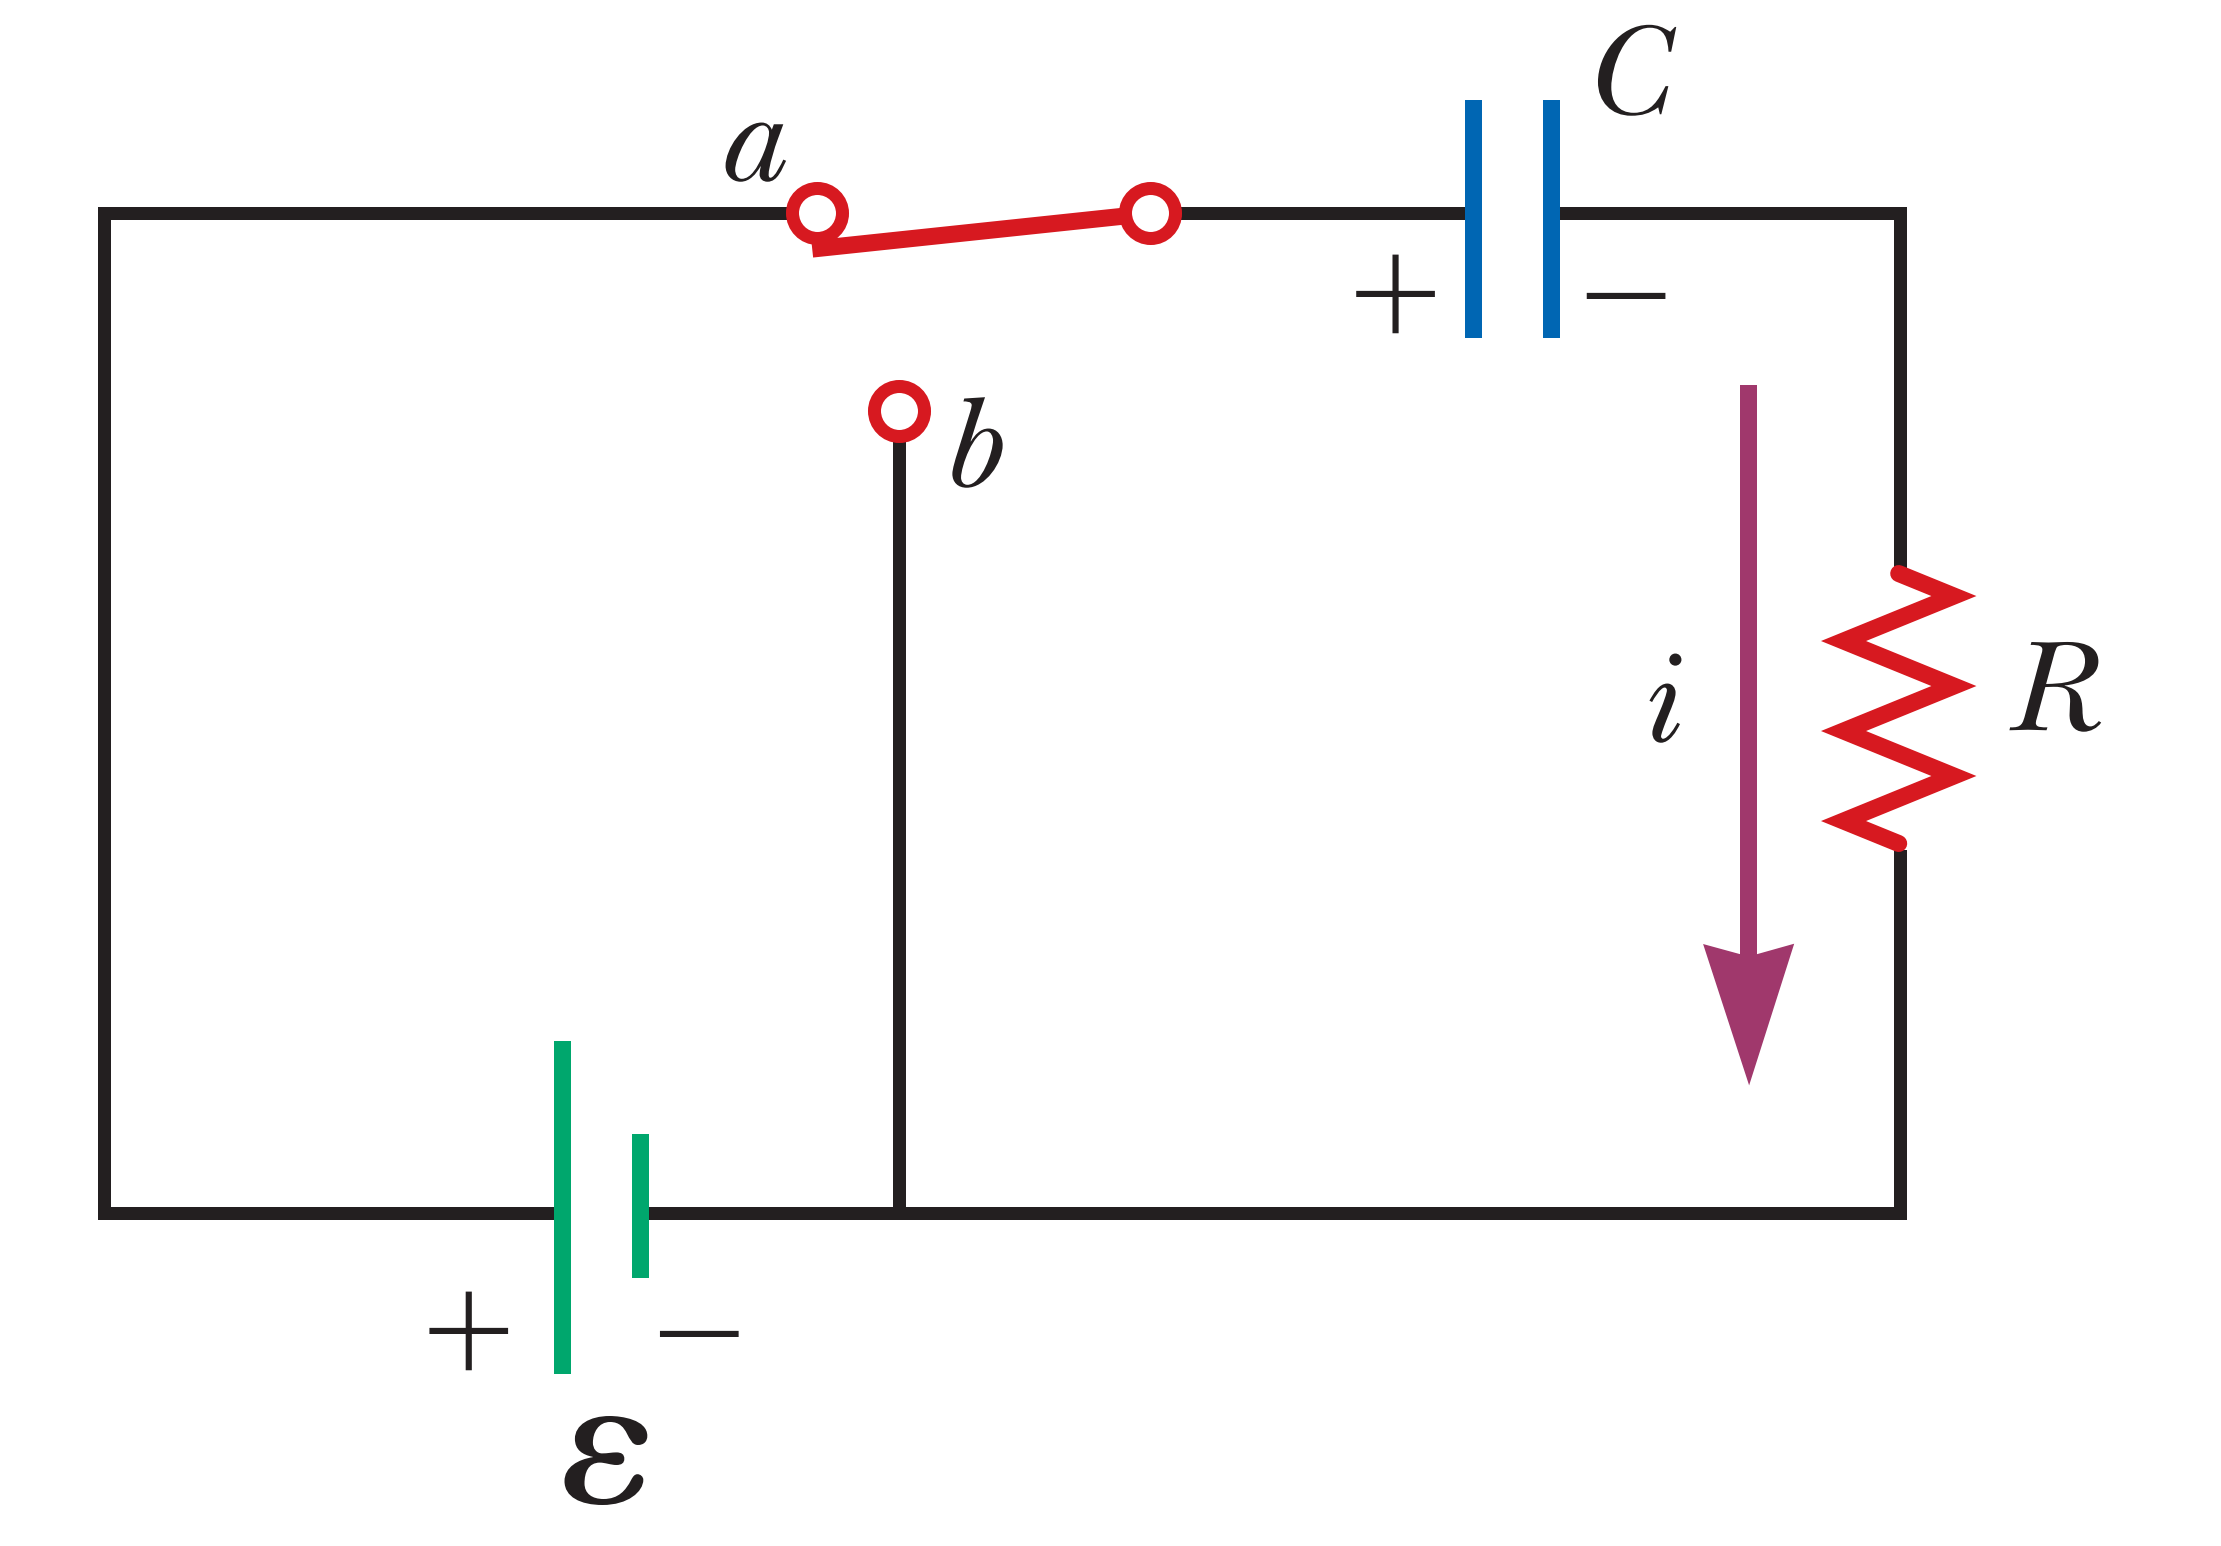
\includegraphics[width=0.4\textwidth]{../Rss/Electromagnetism/Electrodynamics/RCCirc.png}
    \caption*{Figure: RC Circuit}
\end{figure*}

\subsubsection*{RL Circuits.} 
\begin{figure*}[b]
    \centering
    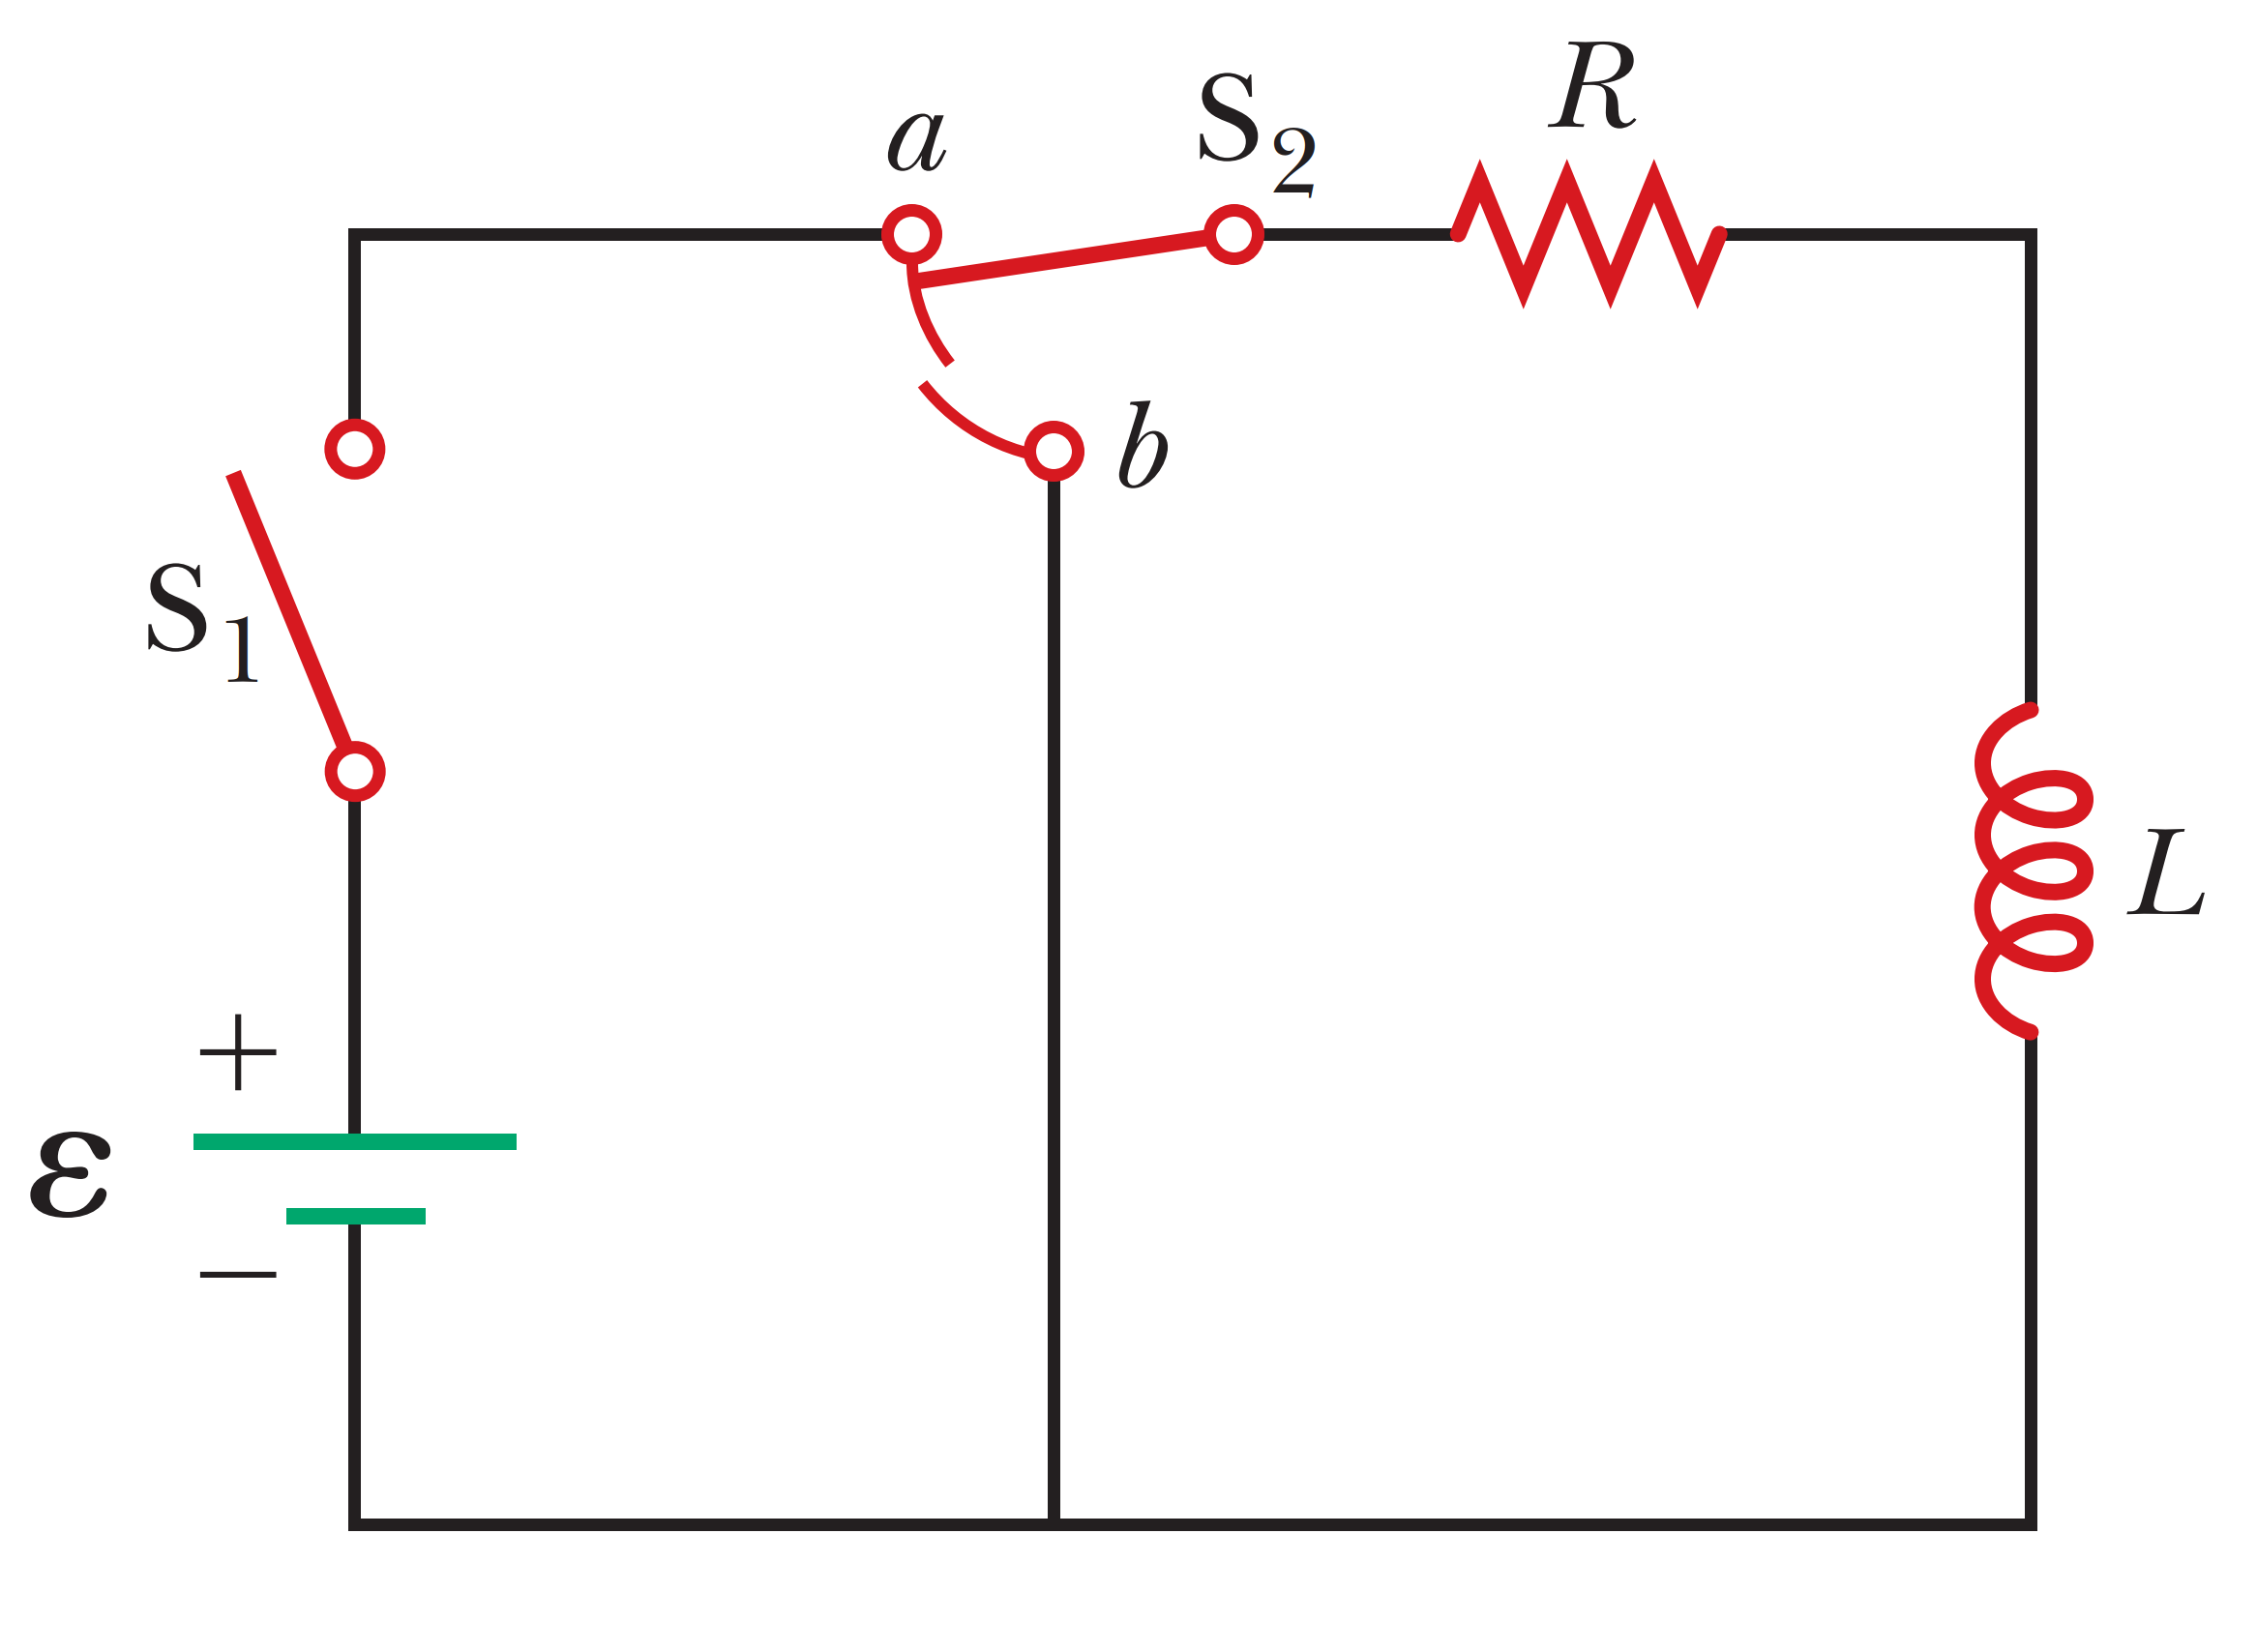
\includegraphics[width=0.4\textwidth]{../Rss/Electromagnetism/Electrodynamics/RLCirc.png}
    \caption*{Figure: RL Circuit}
\end{figure*}
Let’s apply Kirchhoff’s loop rule to the circuit when $S_2$ is set to a and switch $S_1$ is closed
\begin{align*}
    L\dot{i}+iR&=\upvarepsilon\\
    \dot{i}+i\frac{R}{L}&=\frac{\upvarepsilon}{L}
\end{align*}
As before, I use integral factor
\begin{equation*}
    I=\int \frac{R}{L}dt=\frac{R}{L}t
\end{equation*}
Then 
\begin{align*}
    i&=e^{-Rt/L}\int \frac{\upvarepsilon}{L}e^{Rt/L}dt+Ae^{-Rt/L}\\
    i&=\frac{\upvarepsilon}{L}+Ae^{-Rt/L}\\
\end{align*}
Applying boundary condition $i(0) = 0$, we get $A=-\upvarepsilon/R$, thus
\begin{equation*}
    i=\frac{\upvarepsilon}{R}(1-e^{-Rt/L})
\end{equation*}
Since $q= \int i\;dt$
\begin{equation*}
    q=\frac{\upvarepsilon}{R}(1\frac{L}{R}e^{-Rt/L})
\end{equation*}
Now, suppose $S_2$ is thrown from a to b. The differential equation becomes
\begin{equation*}
    \dot{i}+i\frac{R}{L}=0
\end{equation*}
with general solution
\begin{equation*}
    i=Ae^{-Rt/L}
\end{equation*}
Applying boundary condition $i(0) = I_i$, we get $A = I_i$, thus
\begin{equation*}
    i=I_ie^{-Rt/L}
\end{equation*}

\subsubsection*{RLC Circuits.} If the applied voltage varies sinusoidally with time
\begin{equation*}
    v=V_m\sin \omega t
\end{equation*}
then current in the circuit is given by
\begin{equation*}
    i=I_m\sin\omega t-\phi
\end{equation*}
where
\begin{equation*}
    \phi=\arctan^{-1}\frac{Z_{im}}{Z_{Re}}
\end{equation*}
is some phase angle between the current and the applied voltage.
\end{document}
